\documentclass[english,11pt, reqno, oneside]{amsart}
\usepackage{amsmath}
\usepackage{amssymb}
\usepackage[usenames,dvipsnames]{xcolor}
\usepackage[colorlinks=true,linkcolor=blue!95!black, citecolor = green!55!black,bookmarksdepth=3]{hyperref}
\usepackage{tikz}
\usetikzlibrary{calc}
\usetikzlibrary{math}
\usetikzlibrary{decorations.markings, decorations.pathreplacing,shapes.misc}

\begin{document}

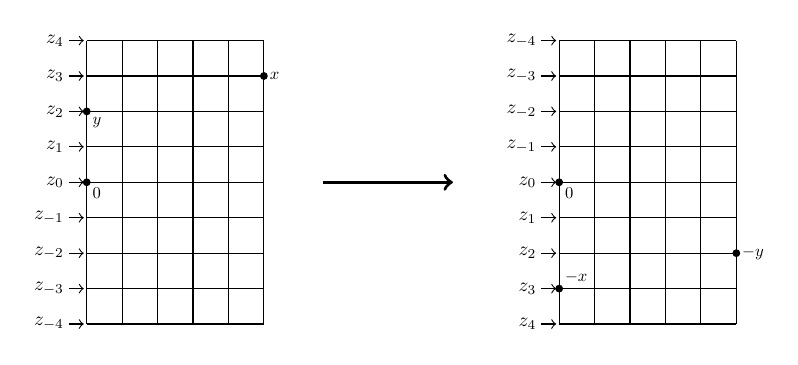
\begin{tikzpicture}[scale=0.75]

\draw (0,-2.405) grid[step=0.6] (3,2.4);

\node[circle, fill, inner sep=1pt] at (0,0) {};
\node[anchor=north west, scale=0.6] at (0,0) {$0$};

\node[circle, fill, inner sep=1pt] at (0,1.2) {};
\node[anchor=north west, scale=0.6] at (0,1.2) {$y$};

\node[circle, fill, inner sep=1pt] at (3, 1.8) {};
\node[anchor=west, scale=0.6] at (3,1.8) {$x$};

\foreach \x in {-4, ..., 4}
{
  \node[anchor=east, scale=0.7] at (-0.27, \x*0.6) {$z_{\x}$};
  \draw[->] (-0.3, \x*0.6) -- ++(0.25,0);
}

\draw[->, very thick] (4,0) -- ++(2.2,0);

\begin{scope}[shift={(8,0)}]
\draw (0,-2.405) grid[step=0.6] (3,2.4);

\node[circle, fill, inner sep=1pt] at (0,0) {};
\node[anchor=north west, scale=0.6] at (0,0) {$0$};

\node[circle, fill, inner sep=1pt] at (3,-1.2) {};
\node[anchor=west, scale=0.6] at (3,-1.2) {$-y$};

\node[circle, fill, inner sep=1pt] at (0, -1.8) {};
\node[anchor=south west, scale=0.6] at (0,-1.8) {$-x$};

\foreach \x in {-4, ..., 4}
{
  \node[anchor=east, scale=0.7] at (-0.27, -\x*0.6) {$z_{\x}$};
  \draw[->] (-0.3, -\x*0.6) -- ++(0.25,0);
}
\end{scope}
\end{tikzpicture}

\end{document}